\documentclass[acmsmall,screen,nonacm]{acmart}
\usepackage[greek,english]{babel}
\usepackage{float}

\babelfont[greek]{rm}{Times New Roman}
\babelfont[greek]{sf}{Arial}
\sloppy


\title{Project 1: Safe Mobile Robot Button Navigation (Ομάδα 1)}


\author{Εμμανουήλ Παξιμαδάκης 1100972 \& Δημήτριος Φιλόπουλος 1101130}
\affiliation{
	\institution{\newline Τμήμα ΗΜ\&ΤΥ, Πανεπιστήμιο Πατρών}
	\country{Ελλάδα}
}
\captionsetup[table]{position=bottom}

\renewcommand{\shortauthors}{Ε.Π., Δ.Φ.}

\begin{document}
	\maketitle
	
	
	\tableofcontents
	
	\newpage
	
	\section{Εισαγωγή}
	Στο πλαίσιο της παρούσας εργασίας, μελετάται το πρόβλημα της ασφαλούς πλοήγησης ενός αυτόνομου κινητού ρομπότ σε ένα δυναμικό περιβάλλον με εμπόδια. Συγκεκριμένα, καλούμαστε να σχεδιάσουμε και να αξιολογήσουμε έναν ελεγκτή πλοήγησης για ένα αυτόνομο όχημα τύπου Racecar στο περιβάλλον \texttt{SafetyRacecarButton2-v0} της βιβλιοθήκης Safety Gymnasium. Ο πρωταρχικός στόχος του οχήματος είναι να κινηθεί και να ενεργοποιήσει διαδοχικά τους σωστούς στόχους, ελαχιστοποιώντας ταυτόχρονα την αύξηση του κόστους που προκύπτει από την επαφή με εμπόδια (hazards) και κινούμενους εχθρούς (gremlins).
	
	Για την επίλυση του προβλήματος και την επαλήθευση των αποτελεσμάτων, αναπτύχθηκαν και συγκρίθηκαν τρεις διαφορετικές προσεγγίσεις:
	\begin{enumerate}
		\item \textbf{Scripted Controller:} Ένας Rule-Based ελεγκτής, ο οποίος λαμβάνει αποφάσεις πλοήγησης και αποφυγής εμποδίων αναλύοντας απευθείας τις μετρήσεις των αισθητήρων Lidar του οχήματος.
		\item \textbf{Simple PPO:} Μια προσέγγιση Ενισχυτικής Μάθησης η οποία βελτιστοποιεί αποκλειστικά reward, αγνοώντας το κόστος.
		\item \textbf{PPO-Lagrangian:} Μια ασφαλής προσέγγιση του PPO η οποία χρησιμοποιεί πολλαπλασιαστές Lagrange για να εξισορροπήσει δυναμικά τη μεγιστοποίηση του reward με την ελαχιστοποίηση του κόστους.
	\end{enumerate}

	\subsection{Εργαλεία και Βιβλιοθήκες Ανάπτυξης}
	Για την υλοποίηση και την πειραματική αξιολόγηση του συστήματος χρησιμοποιήθηκε ένα σύγχρονο οικοσύστημα λογισμικού, το οποίο εξασφαλίζει τη φορητότητα και την επαναληψιμότητα των πειραμάτων:
	\begin{itemize}
		\item \textbf{Python 3.11:} Η βασική γλώσσα προγραμματισμού που χρησιμοποιήθηκε.
		\item \textbf{Virtual Environment:} Χρησιμοποιήθηκε για την απομόνωση των εξαρτήσεων κατά την τοπική ανάπτυξη και την αποφυγή συγκρούσεων μεταξύ των εκδόσεων των πακέτων (μόνο σε αρχικά στάδια του πρότζεκτ για την εύρεση σωστής έκδοσης Python και βιβλιοθηκών).
		\item \textbf{Docker:} Όλη η διαδικασία εκπαίδευσης και αξιολόγησης ενσωματώθηκε σε containers, επιτρέποντας την εκτέλεση του κώδικα σε οποιοδήποτε περιβάλλον χωρίς την ύπαρξη conflictions. 
		\item \textbf{Safety Gymnasium:} Το περιβάλλον προσομοίωσης για την υλοποίηση της εργασίας.
		\item \textbf{PyTorch \& Stable-Baselines3 (SB3):} Η βιβλιοθήκη βαθιάς μάθησης και το framework ενισχυτικής μάθησης που χρησιμοποιήθηκαν για την εκπαίδευση των μοντέλων.
		\item \textbf{TensorBoard:} Εργαλείο οπτικοποίησης των μετρικών των μοντέλων.
	\end{itemize}

	\section{Εξοικίωση με Safety Gymnasium}
	Το ρομπότ είναι ένα Racecar, το οποίο ελέγχεται μέσω ενός πίνακα: $u = [v, \theta]^T$, όπου $v$ είναι η επιθυμητή ταχύτητα των πίσω τροχών και $\theta$ είναι η γωνία διεύθυνσης των μπροστινών τροχών.	Η ανατροφοδότηση που λαμβάνει ο agent από το περιβάλλον σε κάθε χρονικό βήμα αποτελείται από μια εξάδα τιμών: \texttt{(observation, reward, cost, terminated, truncated, info)}. 
	
	Ο χώρος παρατηρήσεων (το observation space) περιλαμβάνει μετρήσεις από διάφορους αισθητήρες, όπως:
	\begin{itemize}
		\item \textbf{Accelerometer, Velocimeter, Gyro, Magnetometer:} Αισθητήρες που καταγράφουν την εσωτερική κατάσταση του οχήματος.
		\item \textbf{Lidar Sensors (Goal, Buttons, Hazards, Gremlins):} Ψευδο-Lidar αισθητήρες 16 κατευθύνσεων (ένας αισθητήρας για κάθε αντικείμενο). Κάθε αισθητήρας επιστρέφει μια τιμή που υποδηλώνει την απόσταση του αντίστοιχου αντικειμένου σε μια συγκεκριμένη κατεύθυνση.
	\end{itemize}
	
	Για τη σταθεροποίηση και τη βελτίωση της εκπαίδευσης των νευρωνικών δικτύων, εφαρμόστηκαν κατάλληλοι μετασχηματιστές στο περιβάλλον, όπως για την κανονικοποίηση των παρατηρήσεων, την εξομάλυνση των ενεργειών του αυτοκινήτου για την αποφυγή απότομων αλλαγών πορείας, και το frame stacking για την αντίληψη της χρονικής εξέλιξης της κίνησης.

	\begin{figure}[H]
		\centering
		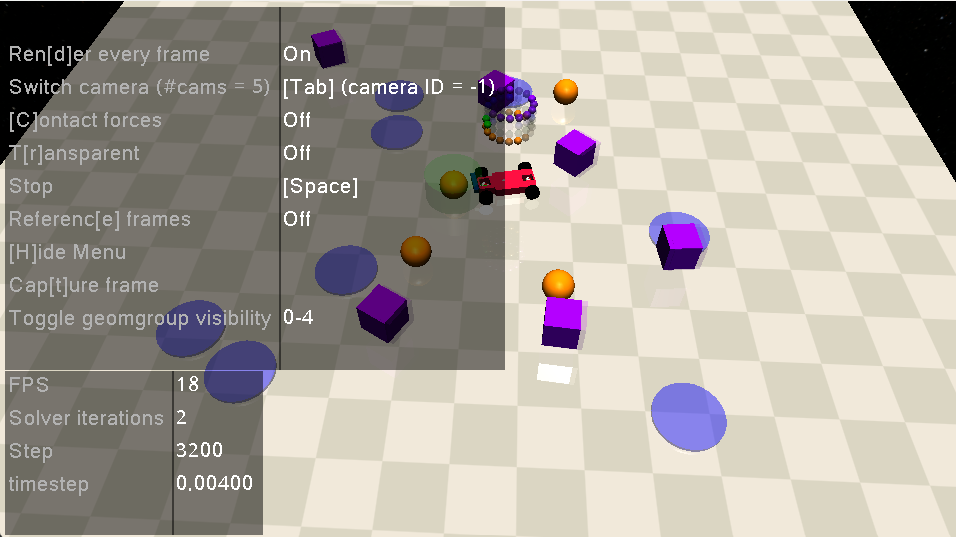
\includegraphics[width=0.8\linewidth]{safety_gymnasium.png}
		\caption{Περιβάλλον Safety Gymnasium}
		\label{fig:safety_gymnasium}
	\end{figure}

	\section{Αρχιτεκτονική και Υλοποίηση Λογισμικού}
	Σε αυτή την ενότητα περιγράφεται η δομή και η αρχιτεκτονική του υλοποιημένου λογισμικού, αναλύοντας πώς συνδέονται τα επιμέρους στοιχεία (δημιουργία περιβάλλοντος, μετασχηματιστές, εκπαίδευση και αξιολόγηση) για την επίλυση του προβλήματος constrained RL.

	\subsection{Δημιουργία και Ρύθμιση Περιβάλλοντος (Environment Setup)}
	Η προετοιμασία του περιβάλλοντος περιλαμβάνει την αρχικοποίηση του βασικού περιβάλλοντος πλοήγησης της βιβλιοθήκης Safety Gymnasium και στη συνέχεια την εφαρμογή μιας σειράς από μετασχηματιστές (wrappers) που σταθεροποιούν την εκπαίδευση, όπως η εξομάλυνση των ενεργειών, η κανονικοποίηση των παρατηρήσεων και η στοίβαξη πλαισίων.

	\subsection{Διαδικασία Εκπαίδευσης και Στοίβα Μετασχηματιστών}
	Για την εκπαίδευση του αλγορίθμου PPO-Lagrangian, το περιβάλλον περιβάλλεται από μια ιεραρχική στοίβα μετασχηματιστών. Η ροή μιας ενέργειας από τον agent προς το περιβάλλον και η επιστροφή των σημάτων (observation, reward, cost) προς τα πίσω ακολουθεί την εξής σειρά:
	
	\begin{enumerate}
		\item \textbf{Λήψη Ενέργειας από τον Agent:} Ο πράκτορας παράγει μια ενέργεια $a_t$, η οποία εισέρχεται στη στοίβα.
		\item \textbf{Action Smoothing:} Ο μετασχηματιστής για το action smoothing εφαρμόζει τον τύπο Exponential Moving Average (EMA) στην ενέργεια για την αποφυγή απότομων αλλαγών κατεύθυνσης και ταχύτητας:
		\begin{equation}
			a_{t,\text{smooth}} = \alpha \cdot a_t + (1 - \alpha) \cdot a_{t-1,\text{smooth}}
		\end{equation}
		\item \textbf{Εκτέλεση Προσομοίωσης:} Δημιουργείται ένα step στον περιβάλλον μεταβιβάζοντας το στην επόμενη κατάσταση. Το περιβάλλον επιστρέφει μια \textbf{εξάδα (6-tuple)} τιμών: 
		\begin{equation}
			(s_t, r_t, c_t, \text{terminated}, \text{truncated}, \text{info})
		\end{equation}
		όπου $s_t$ είναι η παρατήρηση, $r_t$ το reward και $c_t$ το κόστος.
		\item \textbf{Cost Tracking:} Ο μετασχηματιστής καταγραφής κόστους λαμβάνει το 6-tuple και ενημερώνει τις μετρικές του επεισοδίου (συνολικό κόστος, βήματα).
		\item \textbf{Shaped Reward:} Ο μετασχηματιστής Lagrangian λαμβάνει το 6-tuple και υπολογίζει το νέο reward αφαιρώντας το κόστος με βάση τον τρέχοντα πολλαπλασιαστή Lagrange $\beta$:
		\begin{equation}
			r_{t,\text{shaped}} = r_t - \beta \cdot c_t
		\end{equation}
		Η τιμή $\beta$ ενημερώνεται δυναμικά από τη διαδικασία ελέγχου της εκπαίδευσης. Ο μετασχηματιστής αντικαθιστά την αρχική ανταμοιβή $r_t$ με την $r_{t,\text{shaped}}$ στο 6-tuple.
		\item \textbf{Observation Normalization:} Ο μετασχηματιστής κανονικοποίησης παρατηρήσεων λαμβάνει το τροποποιημένο 6-tuple. Υπολογίζει online τον μέσο όρο και τη διασπορά των παρατηρήσεων (μέθοδος Welford) και τις κανονικοποιεί, επιστρέφοντας την κανονικοποιημένη παρατήρηση $\hat{s}_t$:
		\begin{equation}
			\hat{s}_t = \text{clip}\left(\frac{s_t - \mu}{\sqrt{\sigma^2 + \epsilon}}, -10, 10\right)
		\end{equation}
		Αυτό είναι απαραίτητο διότι το περιβάλλον περιλαμβάνει αισθητήρες με πολύ διαφορετικές κλίμακες (π.χ. Lidar $[0, 1]$ και επιταχυνσιόμετρο $[-10, 10]$).
		\item \textbf{Προσαρμογή στο Gymnasium API:} Επειδή το framework εκπαίδευσης αναμένει το κλασικό Gymnasium API με 5 μεταβλητές (όσες έχουμε στο 6-tuple χωρίς το κόστος), ο μετασχηματιστής προσαρμογής του API αφαιρεί το κόστος ($c_t$) από την έξοδο και επιστρέφει:
		\begin{equation}
			(\hat{s}_t, r_{t,\text{shaped}}, \text{terminated}, \text{truncated}, \text{info})
		\end{equation}
		\item \textbf{Καταγραφή Μετρικών (Monitor):} Ο μετασχηματιστής καταγραφής λαμβάνει το 5-tuple, καταγράφει τις μετρικές του επεισοδίου για το εργαλείο οπτικοποίησης και τις προωθεί στον agent.
	\end{enumerate}

	\subsection{Ενδιάμεση Αξιολόγηση κατά την Εκπαίδευση (Evaluation Process)}
	Η ενδιάμεση αξιολόγηση πραγματοποιείται κατά τη διάρκεια της εκπαίδευσης. Κάθε ορισμένο αριθμό βημάτων εκπαίδευσης (έχουμε ορίσει ως προεπιλεγμένη τιμή 10.000 βήματα), η διαδικασία εκτελεί τις εξής ενέργειες:
	\begin{itemize}
		\item \textbf{Συγχρονισμός Στατιστικών Κανονικοποίησης:} Αντιγράφει τις τρέχουσες στατιστικές παραμέτρους (μέση τιμή, διασπορά, πλήθος δειγμάτων) της κανονικοποίησης των παρατηρήσεων από το περιβάλλον εκπαίδευσης στο περιβάλλον αξιολόγησης. 
		\item \textbf{Εκτέλεση Αξιολόγησης:} Εκτελεί ένα deterministic policy στο περιβάλλον αξιολόγησης για ένα σύνολο επεισοδίων.
		\item \textbf{Αποθήκευση Μοντέλου:} Εάν η ανταμοιβή αξιολόγησης είναι καλύτερη από κάθε προηγούμενη, το μοντέλο αποθηκεύεται ως το βέλτιστο μοντέλο.
	\end{itemize}

	\subsection{Ανεξάρτητη Αξιολόγηση}
	Η ανεξάρτητη μονάδα αξιολόγησης χρησιμοποιείται για την τελική σύγκριση των controllers (Rule-Based, Simple PPO, PPO-Lagrangian) σε άγνωστες συνθήκες. Λειτουργεί ως εξής:
	\begin{itemize}
		\item Φορτώνει το εκπαιδευμένο μοντέλο και τις αποθηκευμένες στατιστικές παραμέτρους της κανονικοποίησης των παρατηρήσεων.
		\item Δημιουργεί ένα νέο περιβάλλον αξιολόγησης στο οποίο οι στατιστικές κανονικοποίησης είναι σταθερές (frozen) και δεν ενημερώνονται πλέον.
		\item Εκτελεί τον ελεγκτή για $N=20$ ανεξάρτητα επεισόδια χρησιμοποιώντας συγκεκριμένα random seeds.
		\item Υπολογίζει τις επίσημες μετρικές του πρότζεκτ, όπως τη μέση ανταμοιβή, το μέσο κόστος παραβίασης, το ποσοστό ασφαλών επεισοδίων ($Cost \le 25.0$) και το συνδυασμένο σκορ (Combined Score):
		\begin{equation}
			\text{Score} = \text{Mean Reward} - 1.0 \cdot \text{Mean Cost}
		\end{equation}
	\end{itemize}

	\subsection{Καταγραφή και Οπτικοποίηση με χρήση TensorBoard}
	Για την παρακολούθηση της διαδικασίας εκπαίδευσης και τη διάγνωση της σύγκλισης των μοντέλων, ενσωματώθηκε το TensorBoard. Κατά τη διάρκεια της εκπαίδευσης, μερικές μετρικές που καταγράφονται σε real-time, είναι οι ακόλουθες:
	\begin{itemize}
		\item Η μέση ανταμοιβή ανά επεισόδιο.
		\item Το μέσο κόστος ανά επεισόδιο.
		\item Οι επιμέρους απώλειες του δικτύου, όπως το value loss και το policy loss.
		\item Η δυναμική εξέλιξη του πολλαπλασιαστή Lagrange $\beta$ για το μοντέλο PPO-Lagrangian.
	\end{itemize}

	\section{Δημιουργία Scripted Controller}
	Για τη δημιουργία ενός baseline και για την κατανόηση της δυναμικής του περιβάλλον, σχεδιάστηκε και υλοποιήθηκε ένας Scripted Controller. Η λογική του ελεγκτή βασίζεται στην ανάλυση των σημάτων Lidar και χωρίζεται στα εξής στάδια:
	\begin{enumerate}
		\item \textbf{Ανίχνευση Στόχου:} Ο agent εντοπίζει την κατεύθυνση του επιθυμητού κουμπιού βρίσκοντας το μέγιστο σήμα στον αισθητήρα \texttt{goal\_lidar}. 
		\item \textbf{Διαχωρισμός Εμποδίων:} Για την αποφυγή συγκρούσεων, ο ελεγκτής συνδυάζει τις μετρήσεις των αισθητήρων \texttt{hazards\_lidar}, \texttt{gremlins\_lidar} και των \textit{λανθασμένων} κουμπιών (\texttt{buttons\_lidar} εξαιρώντας την κατεύθυνση του τρέχοντος στόχου) σε έναν ενιαίο χάρτη εμποδίων.
		\item \textbf{Επιλογή Κατεύθυνσης Κίνησης (Gear Selection):} Αν ο στόχος βρίσκεται πίσω από το όχημα, το όχημα κατευθύνεται προς τα πίσω, ενώ στην αντίθετη περίπτωση μπροστά.
		\item \textbf{Αποφυγή Εμποδίων:} Η ανίχνευση εμποδίων γίνεται στις 2 κατευθύνσεις κίνησης. Αν ανιχνευθεί εμπόδιο σε απόσταση μικρότερη από ένα όριο ασφαλείας στην κατεύθυνση κίνησης, ο agent στρίβει κατάλληλα μακριά από το εμπόδιο (επιλέγοντας την πλευρά με το μικρότερο κόστος εμποδίων), ενώ παράλληλα μειώνει την ταχύτητά του.
	\end{enumerate}
	
	\subsection{Αποτελέσματα και Ανάλυση}
	Ο σχεδιασμένος Scripted Controller αξιολογήθηκε στο περιβάλλον \texttt{SafetyRacecarButton2-v0} για $20$ ανεξάρτητα επεισόδια για διάφορα seeds. Κάθε επεισόδιο είχε μέγιστη διάρκεια $1000$ βήματα. Τα συγκεντρωτικά αποτελέσματα της αξιολόγησης παρουσιάζονται στον Πίνακα~\ref{tab:scripted_results}.

	\begin{table}[H]
		\centering
		\begin{tabular}{lc}
			\toprule
			\textbf{Μετρική} & \textbf{Τιμή / Επίδοση} \\
			\midrule
			Αριθμός Επεισοδίων & 20 \\
			Μέση Ανταμοιβή & $+3.1368 \pm 2.5198$ \\
			Ελάχιστη / Μέγιστη Ανταμοιβή & $[+0.1886, +9.0047]$ \\
			Μέσο Κόστος & $202.80 \pm 251.51$ \\
			Μέγιστο Κόστος Επεισοδίου & $819.00$ \\
			Ποσοστό Επεισοδίων με Μηδενικό Κόστος & $10.0\%$ ($2/20$) \\
			Ποσοστό Ασφαλών Επεισοδίων ($Cost \le 25.0$) & $30.0\%$ ($6/20$) \\
			Combined Score ($R - 1.0 \times C$) & $-199.6632$ \\
			\bottomrule
		\end{tabular}
		\caption{Αποτελέσματα Αξιολόγησης του Scripted Controller ($20$ επεισόδια)}
		\label{tab:scripted_results}
	\end{table}

	\subsubsection{Ανάλυση Συμπεριφοράς και Περιορισμών}
	Από την ανάλυση των αποτελεσμάτων και την παρατήρηση της κίνησης του οχήματος, προκύπτουν τα ακόλουθα συμπεράσματα για τη συμπεριφορά του ελεγκτή:
	\begin{itemize}
		\item \textbf{Ικανότητα Πλοήγησης:} Ο ελεγκτής επιτυγχάνει θετική μέση ανταμοιβή ($+3.1368$), γεγονός που δείχνει ότι το όχημα καταφέρνει να εντοπίσει και να χτυπήσει τους επιθυμητούς στόχους.
		\item \textbf{Πρόβλημα Κόστους:} Το μέσο κόστος ασφάλειας είναι εξαιρετικά υψηλό ($202.80$). Το ποσοστό των ασφαλών επεισοδίων είναι μόλις $30.0\%$, ενώ σε ορισμένες περιπτώσεις, το συσσωρευμένο κόστος αγγίζει πολύ υψηλές τιμές.
		\item \textbf{Τοπικά Ελάχιστα:} Σε περιοχές με υψηλή πυκνότητα εμποδίων ή κοντά σε εμπόδια (gremlins/hazards), ο ελεγκτής μπορεί να παρουσιάσει ταλαντώσεις στην κατεύθυνση τιμονιού, με αποτέλεσμα να παγιδεύεται και να συγκρούεται συνεχόμενα με το ίδιο εμπόδιο.
	\end{itemize}

	\begin{figure}[H]
		\centering
		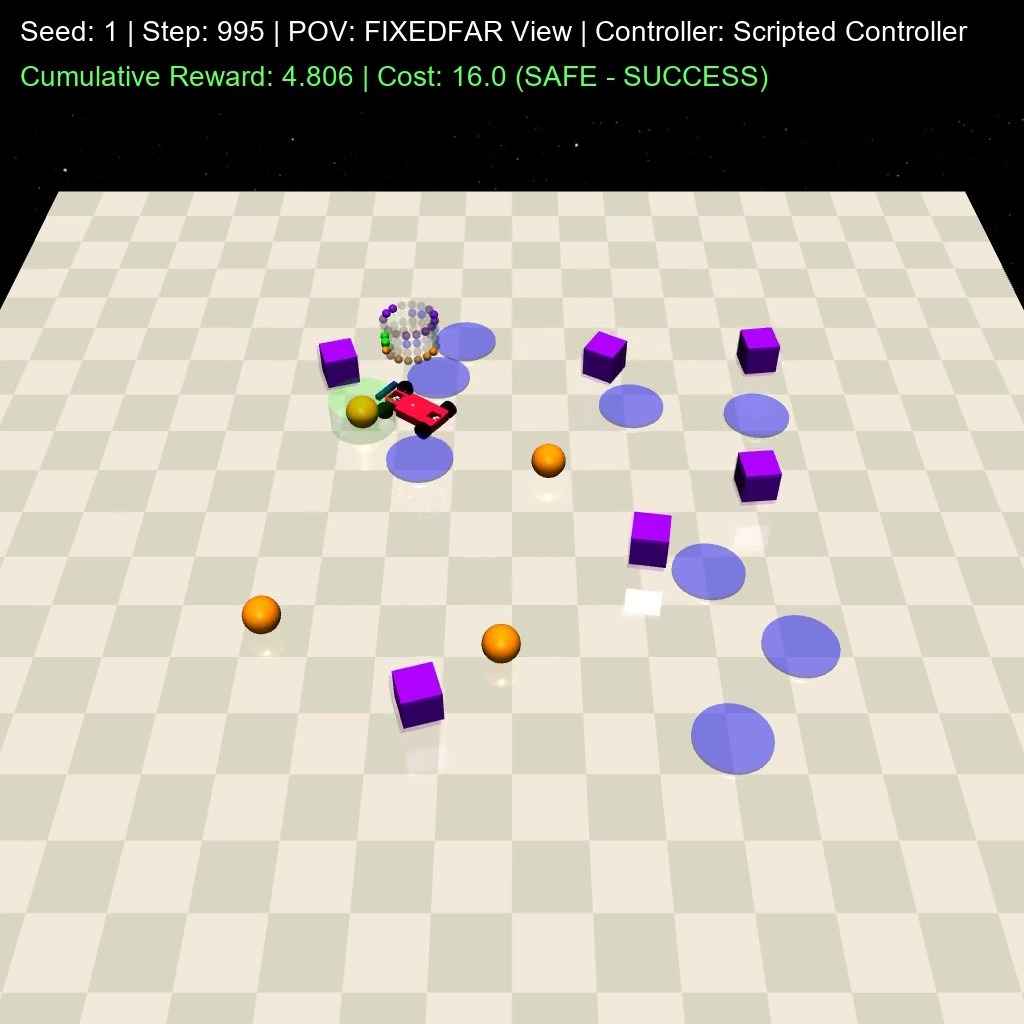
\includegraphics[width=0.7\linewidth]{scripted_success.jpg}
		\caption{Παράδειγμα επιτυχούς πλοήγησης (Success Seed Case) του Scripted Controller (Seed 1).}
		\label{fig:scripted_success}
	\end{figure}

	\begin{figure}[H]
		\centering
		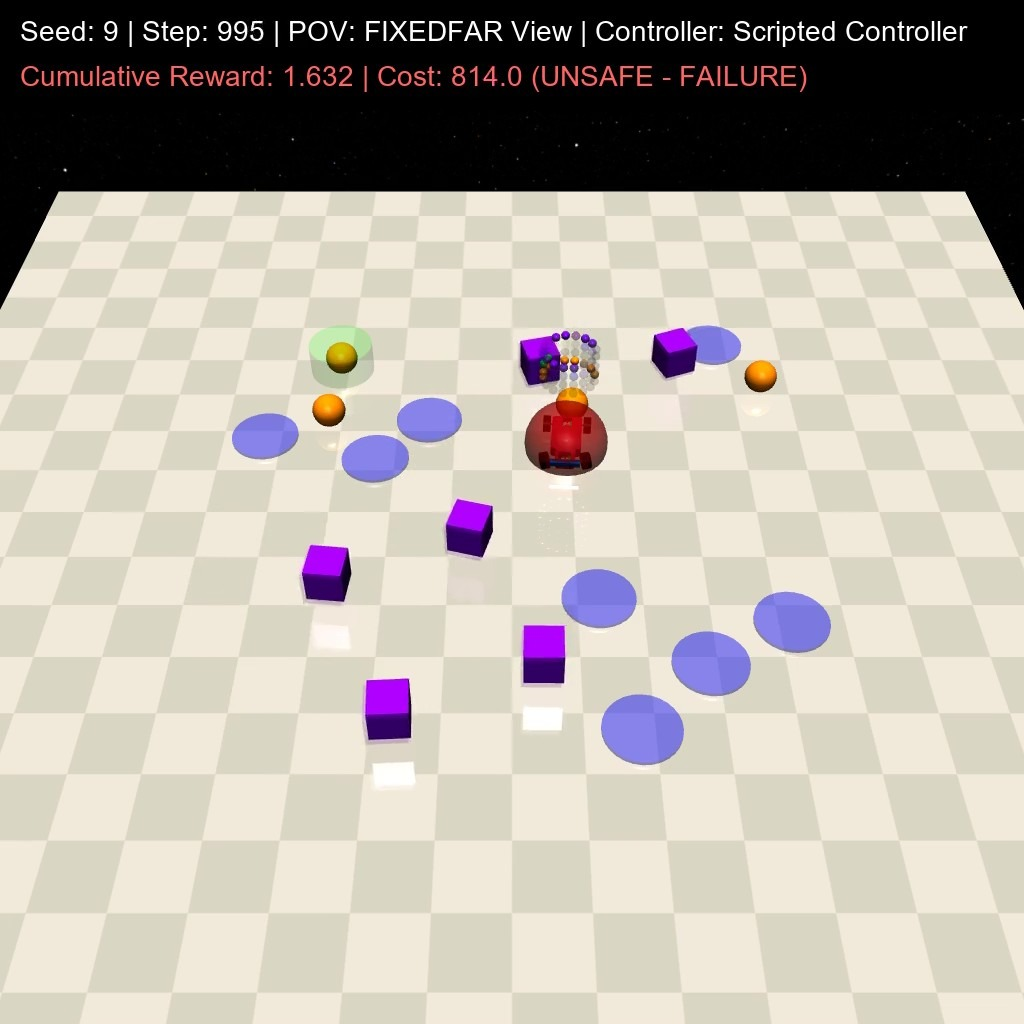
\includegraphics[width=0.7\linewidth]{scripted_failure.jpg}
		\caption{Παράδειγμα αποτυχίας πλοήγησης (Failure Seed Case) του Scripted Controller (Seed 9).}
		\label{fig:scripted_failure}
	\end{figure}
	
	\section{Simple PPO (Reward-only Baseline)}
	Για μια πρώτη προσέγγιση του προβλήματος βασιστήκαμε στον αλγόριθμο \textbf{Proximal Policy Optimization (PPO)}, ένας on-policy αλγόριθμος που λειτουργεί σε συνεχή χώρο ενεργειών.
	Ο Simple PPO χρησιμοποιείται ως \textbf{Reward-only Baseline}. Αυτό σημαίνει ότι ο πράκτορας εκπαιδεύεται μόνο για την μεγιστοποίηση του reward function, αγνοώντας πλήρως το κόστος που προκύπτει από τις συγκρούσεις με εμπόδια (hazards ή gremlins).

	\subsection{Θεωρητικό Υπόβαθρο}
	Ο αλγόριθμος Proximal Policy Optimization (PPO) αποτελεί μία μέθοδο Policy Gradient. Έχει ως στόχο να προσεγγίσει τη σταθερότητα και την απόδοση της μεθόδου Trust Region Policy Optimization (TRPO), αλλά χωρίς την πολυπλοκότητα των περιορισμών της, γεγονός που τον καθιστά ευκολότερο στην υλοποίηση και στην εφαρμογή σε μεγάλα νευρωνικά δίκτυα, οπως το δικό μας.

	Γι' αυτό ο PPO εισάγει μια ειδική αντικειμενική συνάρτηση η οποία κάνει clip τις αλλαγές στο policy, ώστε η νέα policy $\pi_\theta$ να μην αποκλίνει σημαντικά από την προηγούμενη $\pi_{\theta_{\text{old}}}$. Η συνάρτηση στόχου του PPO ορίζεται ως:
	\begin{equation}
		J(\theta) = \mathbb{E} \left[ \min \left( v_{\text{ratio}} A(s, a), \, \text{clip}(v_{\text{ratio}}, 1 - \epsilon, 1 + \epsilon) A(s, a) \right) \right]
	\end{equation}
	όπου:
	\begin{itemize}
		\item $v_{\text{ratio}} = \frac{\pi_\theta(s, a)}{\pi_{\theta_{\text{old}}}(s, a)}$ είναι ο λόγος πιθανοτήτων (probability ratio) που δείχνει πόσο πιο πιθανή είναι η ενέργεια $a$ στην κατάσταση $s$ υπό τη νέα πολιτική $\pi_\theta$ σε σχέση με την παλιά $\pi_{\theta_{\text{old}}}$.
		\item $A(s, a)$ είναι η συνάρτηση πλεονεκτήματος (advantage function).
		\item $\epsilon$ είναι η παράμετρος αποκοπής (clipping parameter), η οποία περιορίζει τις τιμές του λόγου $v_{\text{ratio}}$ στο διάστημα $[1 - \epsilon, \, 1 + \epsilon]$.
	\end{itemize}

	Με το clipping δεν έχουμε καταστροφικά μεγάλα βήματα ενημέρωσης των παραμέτρων της policy. Αν η νέα πολιτική βελτιώνει σημαντικά την επίδοση αλλά απομακρύνεται υπερβολικά από την παλιά, η συνάρτηση $\text{clip}$ σταθεροποιεί την αντικειμενική τιμή, αποτρέποντας περαιτέρω αλλαγές. 

	Στην πράξη, η τελική συνάρτηση στόχου που βελτιστοποιείται από τον PPO περιέχει συνήθως επιπλέον όρους:
	\begin{itemize}
		\item \textbf{Value Function Approximation Loss:} Έναν όρο σφάλματος για την εκπαίδευση του critic, ο οποίος εκτιμά τη συνάρτηση αξίας $V(s)$.
		\item \textbf{Policy Entropy:} Έναν όρο εντροπίας της πολιτικής που ενθαρρύνει την εξερεύνηση (exploration) του χώρου ενεργειών και αποτρέπει την πρόωρη σύγκλιση σε τοπικά βέλτιστα.
	\end{itemize}

	\subsection{Διαδικασία και Παράμετροι Εκπαίδευσης}
	Η εκπαίδευση του απλού PPO πραγματοποιήθηκε με χρήση της βιβλιοθήκης \texttt{Stable-Baselines3} (SB3). Για τη βελτιστοποίηση της μάθησης και τη σταθεροποίηση του νευρωνικού δικτύου, εφαρμόστηκε η ακόλουθη διαδικασία:
	\begin{itemize}
		\item \textbf{Κανονικοποίηση Παρατηρήσεων:} Χρησιμοποιήθηκε ένας μετασχηματιστής κανονικοποίησης παρατηρήσεων ο οποίος υπολογίζει online τον τρέχοντα μέσο όρο και την τυπική απόκλιση των παρατηρήσεων (μέθοδος Welford) και τις κανονικοποιεί στο διάστημα $[-10, 10]$. Αυτό αποτρέπει τον κορεσμό των ενεργοποιήσεων του δικτύου λόγω των μεγάλων διακυμάνσεων των αισθητήρων Lidar.
		\item \textbf{Action Smoothing:} Εφαρμόστηκε ένας μετασχηματιστής εξομάλυνσης ενεργειών με εκθετικό κινητό μέσο όρο (EMA) και συντελεστή $\alpha = 0.8$. Αυτό βοηθά στη μείωση των απότομων αλλαγών στην ταχύτητα και τη γωνία διεύθυνσης, προστατεύοντας το όχημα από ανεξέλεγκτες ολισθήσεις.
		\item \textbf{Αρχιτεκτονική Δικτύου:} Χρησιμοποιήθηκε μια MLP αρχιτεκτονική με δύο κρυφά επίπεδα των 256 νευρώνων το καθένα για τον actor και τον critic.\\
	\end{itemize}
	
	
	Για την εκπαίδευση επιλέξαμε υπερπαράμετροι που ευνοούν τη μεγιστοποίηση της ανταμοιβής. Συγκεκριμένα, επιθυμούμε μεγάλο αριθμό \texttt{N Steps} και μεγάλο \texttt{Batch Size}, καθώς η απουσία περιορισμών ασφαλείας μάς επιτρέπει να συλλέγουμε μεγαλύτερα δείγματα εμπειρίας για πιο αξιόπιστες εκτιμήσεις της πολιτικής. Παράλληλα, χρησιμοποιείται μια μικρή τιμή στο συντελεστή εντροπίας για την ενθάρρυνση της εξερεύνησης, αποτρέποντας τον πράκτορα από το να κολλήσει πρόωρα σε τοπικά μέγιστα.\\

	Οι βασικές υπερπαράμετροι της εκπαίδευσης παρουσιάζονται στον Πίνακα~\ref{tab:ppo_unconstrained_hyperparams}.

	\begin{table}[H]
		\centering
		\begin{tabular}{lc}
			\toprule
			\textbf{Υπερπαράμετρος} & \textbf{Τιμή} \\
			\midrule
			Συνολικά Βήματα Εκπαίδευσης & 3.000.000 \\
			Ρυθμός Μάθησης & $3 \times 10^{-4}$ \\
			Batch Size & 512 \\
			N Steps & 4096 \\
			Αριθμός Εποχών & 10 \\
			Συντελεστής $\gamma$ & 0.99 \\
			Παράμετρος Αποκοπής ($\epsilon$) & 0.2 \\
			Συντελεστής Εντροπίας & 0.02 \\
			\bottomrule
		\end{tabular}
		\caption{Υπερπαράμετροι Εκπαίδευσης του Simple PPO}
		\label{tab:ppo_unconstrained_hyperparams}
	\end{table}

	\subsection{Αποτελέσματα}
	Τα αποτελέσματα της αξιολόγησης του εκπαιδευμένου Simple PPO μοντέλου για 20 επεισόδια και μήκος βήματος 1000 παρουσιάζονται στον Πίνακα~\ref{tab:ppo_unconstrained_results}.

	\begin{table}[H]
		\centering
		\begin{tabular}{lc}
			\toprule
			\textbf{Μετρική} & \textbf{Τιμή / Επίδοση} \\
			\midrule
			Αριθμός Επεισοδίων & 20 \\
			Μέση Ανταμοιβή & $+2.8220 \pm 2.3994$ \\
			Ελάχιστη / Μέγιστη Ανταμοιβή & $[-0.0631, +9.5873]$ \\
			Μέσο Κόστος Ασφάλειας  & $170.85 \pm 205.60$ \\
			Μέγιστο Κόστος  & $607.00$ \\
			Ποσοστό Επεισοδίων με Μηδενικό Κόστος & $15.0\%$ ($3/20$) \\
			Ποσοστό Ασφαλών Επεισοδίων ($Cost \le 25.0$) & $30.0\%$ ($6/20$) \\
			Συνδυασμένο Σκορ ($R - 1.0 \times C$) & $-168.0280$ \\
			\bottomrule
		\end{tabular}
		\caption{Αποτελέσματα Αξιολόγησης του Simple PPO Controller}
		\label{tab:ppo_unconstrained_results}
	\end{table}

	\begin{figure}[H]
		\centering
		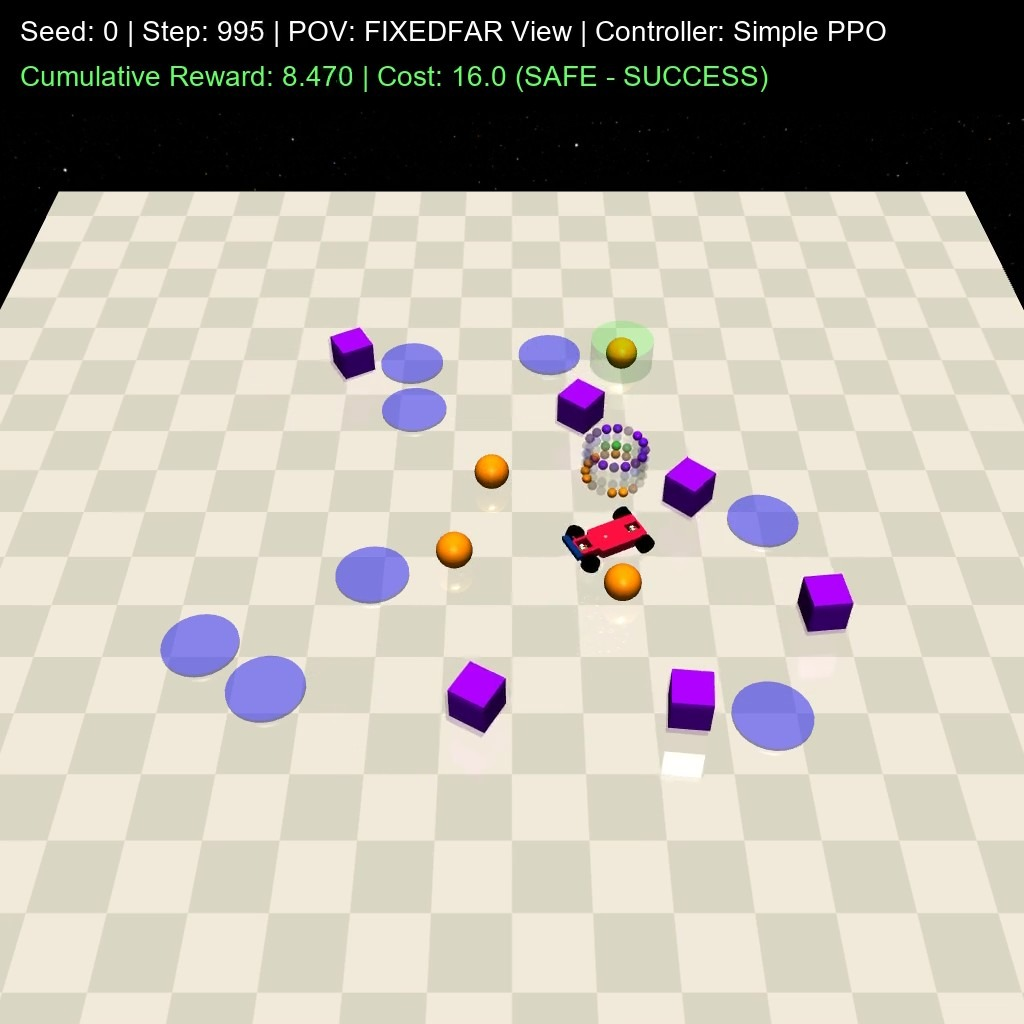
\includegraphics[width=0.7\linewidth]{ppo_simple_success.jpg}
		\caption{Παράδειγμα επιτυχούς πλοήγησης (Success Seed Case) του Simple PPO (Seed 0).}
		\label{fig:ppo_simple_success}
	\end{figure}

	\begin{figure}[H]
		\centering
		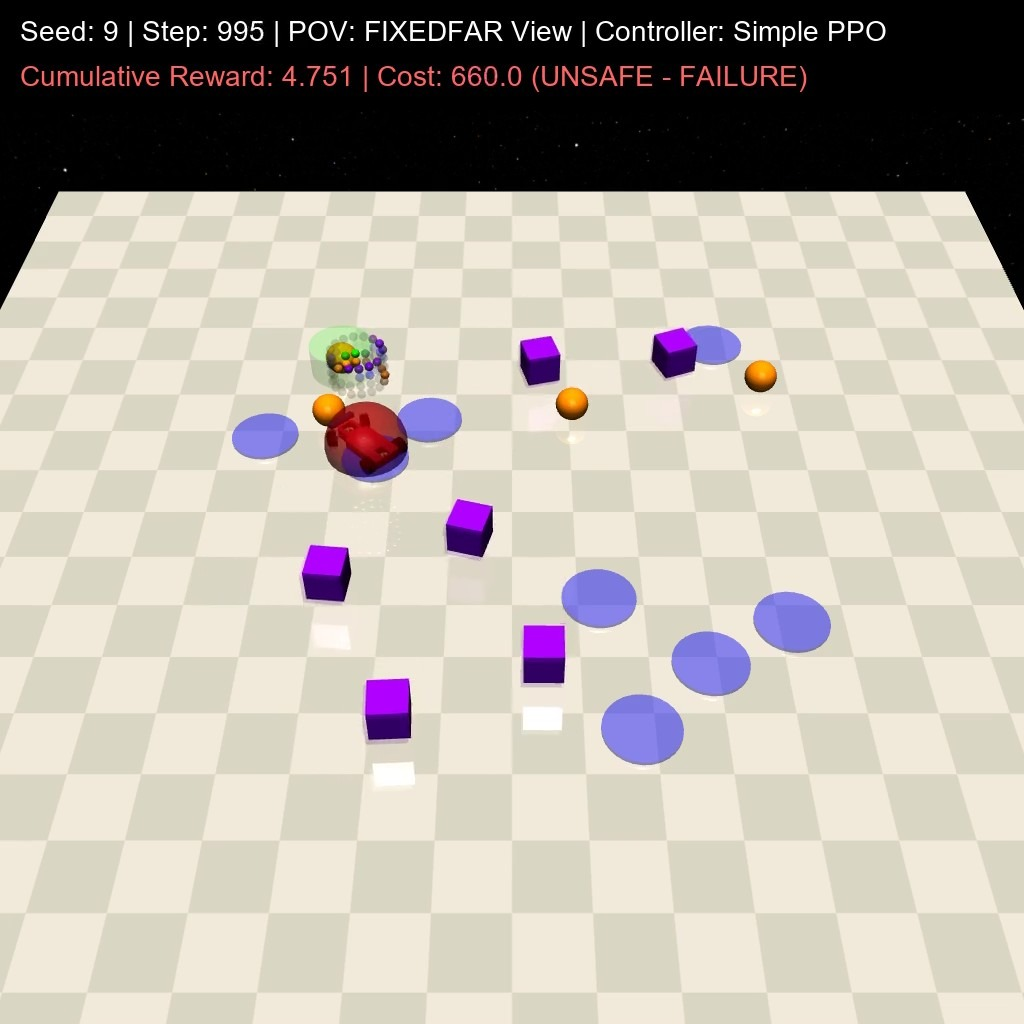
\includegraphics[width=0.7\linewidth]{ppo_simple_failure.jpg}
		\caption{Παράδειγμα αποτυχίας πλοήγησης (Failure Seed Case) του Simple PPO (Seed 9).}
		\label{fig:ppo_simple_failure}
	\end{figure}
	
	\section{Safe Proximal Policy Optimization}
	Για την επίλυση του προβλήματος της ασφάλειας, υλοποιήθηκε μια προσέγγιση \textbf{Constrained Reinforcement Learning} βασισμένη στον PPO αλγόριθμο με χρήση πολλαπλασιαστών Lagrange (\textbf{PPO-Lagrangian}).

	\subsection{Θεωρητικό Υπόβαθρο}
	Το πρόβλημα της ασφαλούς πλοήγησης μοντελοποιείται ως ένα \textit{Περιορισμένο Μαρκοβιανό Πρόγραμμα Αποφάσεων (Constrained Markov Decision Process - CMDP)}. Στόχος είναι να βρούμε μια πολιτική $\pi$ που μεγιστοποιεί την ανταμοιβή, ενώ ταυτόχρονα διασφαλίζει ότι το κόστος ασφάλειας δεν υπερβαίνει ένα όριο $C_{\text{limit}}$:
	\begin{equation}
		\max_{\pi} \mathbb{E} \left[ \sum_{t=0}^{T} \gamma^t r_t \right] \quad \text{subject to} \quad \mathbb{E} \left[ \sum_{t=0}^{T} \gamma^t c_t \right] \le C_{\text{limit}}
	\end{equation}
	Με τους πολλαπλασιαστές Lagrange καταφέρνουμε τη μετατροπή του περιορισμένου αυτού προβλήματος σε ένα ισοδύναμο μη περιορισμένο πρόβλημα βελτιστοποίησης, εισάγοντας έναν θετικό πολλαπλασιαστή $\beta \ge 0$:
	\begin{equation}
		\max_{\pi} \min_{\beta \ge 0} \mathcal{L}(\pi, \beta) = J_R(\pi) - \beta (J_C(\pi) - C_{\text{limit}})
	\end{equation}
	όπου $J_R(\pi)$ είναι η αναμενόμενη ανταμοιβή και $J_C(\pi)$ είναι το αναμενόμενο κόστος. Η βελτιστοποίηση πραγματοποιείται σε δύο επίπεδα:
	\begin{enumerate}
		\item \textbf{Βελτιστοποίηση Πολιτικής ($\pi$):} Η πολιτική εκπαιδεύεται να μεγιστοποιεί τη διαμορφωμένη συνάρτηση στόχου (Lagrangian reward): $r_{\text{shaped}} = r - \beta \cdot c$. Αν ο πολλαπλασιαστής $\beta$ είναι μεγάλος, ο πράκτορας τιμωρείται αυστηρά για κάθε σύγκρουση, στρέφοντας την προσοχή του στην ασφάλεια. Αν $\beta = 0$, ο πράκτορας συμπεριφέρεται όπως ένας κλασικός ελεύθερος περιορισμών πράκτορας.
		\item \textbf{Ενημέρωση Πολλαπλασιαστή ($\beta$):} Ο πολλαπλασιαστής ενημερώνεται δυναμικά στο τέλος κάθε rollout μέσω gradient ascent:
		\begin{equation}
			\beta \leftarrow \max\left(0, \, \beta + \eta \, (J_C(\pi) - C_{\text{limit}})\right)
		\end{equation}
		όπου $\eta$ είναι ο ρυθμός μάθησης της παραμέτρου Lagrange (Lagrangian learning rate). Αν το μέσο κόστος του rollout υπερβαίνει το $C_{\text{limit}}$, το $\beta$ αυξάνεται, εντείνοντας την ποινή ασφάλειας. Αν το κόστος είναι χαμηλότερο από το όριο, το $\beta$ μειώνεται, επιτρέποντας στον πράκτορα να εστιάσει ξανά στη συλλογή ανταμοιβών.
	\end{enumerate}

	\subsection{Διαδικασία και Παράμετροι Εκπαίδευσης}
	Η υλοποίηση βασίζεται στη βιβλιοθήκη \texttt{Stable-Baselines3} με την προσθήκη κατάλληλων μετασχηματιστών (wrappers) και διαδικασιών ελέγχου (callbacks):
	\begin{itemize}
		\item \textbf{Μετασχηματιστής Lagrangian:} Αυτός ο μετασχηματιστής παρεμβάλλεται στο βήμα της προσομοίωσης και τροποποιεί την ανταμοιβή που επιστρέφει το περιβάλλον σε $r_{\text{shaped}} = r - \beta \cdot c$, χρησιμοποιώντας την τρέχουσα τιμή του $\beta$ από τη διαδικασία ελέγχου.
		\item \textbf{Μετασχηματιστής Προσαρμογής API:} Προσαρμόζει το 6-tuple του περιβάλλοντος στο 5-tuple που αναμένει ο αλγόριθμος. Επιπλέον, εισάγει έναν μηχανισμό ασφαλείας: αν το συσσωρευμένο κόστος του επεισοδίου υπερβεί μια τιμή-κατώφλι (π.χ. 50.0), το επεισόδιο τερματίζεται πρόωρα (\texttt{terminated = True}) και επιβάλλεται μια σταθερή ποινή ανταμοιβής $-5.0$, αποτρέποντας τον πράκτορα από το να συνεχίσει να συγκρούεται με εμπόδια.
		\item \textbf{Διαδικασία Ενημέρωσης Lagrange (Callback):} Παρακολουθεί το μέσο κόστος των επεισοδίων σε κάθε κύκλο εμπειριών (rollout) και ενημερώνει δυναμικά την τιμή του $\beta$ σύμφωνα με τον κανόνα ενημέρωσης, καταγράφοντας την εξέλιξή του στο εργαλείο οπτικοποίησης.
		\item \textbf{Διαδικασία Συγχρονισμού Στατιστικών (Callback):} Διασφαλίζει ότι οι online στατιστικές κανονικοποίησης (μέση τιμή/διασπορά) του μετασχηματιστή εκπαίδευσης μεταφέρονται αυτούσιες στο περιβάλλον αξιολόγησης κατά τη διάρκεια των ενδιάμεσων ελέγχων, ώστε να μην διαταράσσεται η συμπεριφορά του ελεγκτή.\\
	\end{itemize}
	
	Στην περίπτωση του \textbf{PPO-Lagrangian}, λόγω των περιορισμών ασφάλειας, έχουμε διαφορετική προσέγγιση στις υπερπαραμέτρους. Αρχικά, θέλουμε μικρότερο αριθμό \texttt{N Steps} και μικρότερο \texttt{Batch Size}, ώστε η ενημέρωση του πολλαπλασιαστή Lagrange ($\beta$) να γίνεται συχνότερα και η πολιτική να προσαρμόζεται άμεσα στις παραβιάσεις. Επιπλέον, εισάγεται το όριο κόστους ($C_{\text{limit}}$), ο ρυθμός μάθησης Lagrange ($\eta$) για ευαισθησία ποινής και ένα μέγιστο όριο πολλαπλασιαστή ($\beta_{\text{max}}$) για την αποφυγή κατάρρευσης της πολιτικής. Τέλος, ο συντελεστής εντροπίας μηδενίζεται για να αποφευχθούν τυχαίες, ριψοκίνδυνες κινήσεις κοντά στα εμπόδια.\\

	Οι βασικές υπερπαράμετροι εκπαίδευσης του PPO-Lagrangian παρουσιάζονται στον Πίνακα~\ref{tab:ppo_lagrangian_hyperparams}.

	\begin{table}[H]
		\centering
		\begin{tabular}{lc}
			\toprule
			\textbf{Υπερπαράμετρος} & \textbf{Τιμή} \\
			\midrule
			Συνολικά Βήματα Εκπαίδευσης & 3.000.000 \\
			Ρυθμός Μάθησης & $3 \times 10^{-4}$ \\
			Batch Size & 64 \\
			N Steps & 2048 \\
			Αριθμός Εποχών &10 \\
			Συντελεστής $\gamma$ & 0.99 \\
			Όριο Κόστους ($C_{\text{limit}}$) & 25.0 \\
			Ρυθμός Μάθησης Lagrange ($\eta$) & 0.02 \\
			Μέγιστη Τιμή Πολλαπλασιαστή ($\beta_{\text{max}}$) & 10.0 \\
			Συντελεστής Εντροπίας & 0.0 \\
			\bottomrule
		\end{tabular}
		\caption{Υπερπαράμετροι Εκπαίδευσης του PPO-Lagrangian}
		\label{tab:ppo_lagrangian_hyperparams}
	\end{table}

	

	\subsection{Αποτελέσματα}
	Τα αποτελέσματα της αξιολόγησης του εκπαιδευμένου PPO-Lagrangian μοντέλου για 20 επεισόδια και για μήκος επεισοδίου 1000 βήματα παρουσιάζονται στον Πίνακα~\ref{tab:ppo_lagrangian_results} (τα δεδομένα θα συμπληρωθούν μετά την ολοκλήρωση της εκπαίδευσης).

	\begin{table}[H]
		\centering
		\begin{tabular}{lc}
			\toprule
			\textbf{Μετρική} & \textbf{Τιμή / Επίδοση} \\
			\midrule
			Αριθμός Επεισοδίων & 20 \\
			Μέση Ανταμοιβή  & \textit{[Υπό Εκπαίδευση]} \\
			Ελάχιστη / Μέγιστη Ανταμοιβή & \textit{[Υπό Εκπαίδευση]} \\
			Μέσο Κόστος Ασφάλειας & \textit{[Υπό Εκπαίδευση]} \\
			Μέγιστο Κόστος Επεισοδίου & \textit{[Υπό Εκπαίδευση]} \\
			Ποσοστό Επεισοδίων με Μηδενικό Κόστος & \textit{[Υπό Εκπαίδευση]} \\
			Ποσοστό Ασφαλών Επεισοδίων ($Cost \le 25.0$) & \textit{[Υπό Εκπαίδευση]} \\
			Συνδυασμένο Σκορ ($R - 1.0 \times C$) & \textit{[Υπό Εκπαίδευση]} \\
			\bottomrule
		\end{tabular}
		\caption{Αποτελέσματα Αξιολόγησης του PPO-Lagrangian Controller}
		\label{tab:ppo_lagrangian_results}
	\end{table}

	

	\section{Συμπεράσματα}
	Για τους ελεγκτές που υλοποιήσαμε μπορούμε να συμπεράνουμε τα εξής:

	\begin{itemize}
		\item Ο \textbf{Scripted Controller} αποτελεί μια απλή και άμεση προσέγγιση, η οποία βασίζεται αποκλειστικά σε Lidar μετρήσεις. Γι' αυτό, παρόλο που καταφέρνει να πλοηγηθεί και να ενεργοποιήσει κουμπιά (μέση ανταμοιβή $+3.1368$), έχει πολύ υψηλό μέσο κόστος.
	\end{itemize}
	

	Στην συνέχεια, οι δύο προσεγγίσεις Ενισχυτικής Μάθησης (Reinforcement Learning) όπως περιμέναμε προσέφεραν αρκετές βελτιώσεις:
	\begin{itemize}
		\item Ο \textbf{Simple PPO (Reward-only Baseline)} επιτυγχάνει ικανοποιητική μέση ανταμοιβή ($+2.8220$), καθώς εκπαιδεύεται να βελτιστοποιεί άμεσα την τροχιά του οχήματος προς τους στόχους. Ωστόσο, επειδή αγνοεί πλήρως τους περιορισμούς ασφάλειας, παρουσιάζει  υψηλό μέσο κόστος ($170.85$), επιβεβαιώνοντας ότι δεν επαρκεί για την περίπτωση μας όπου η ασφάλεια είναι κρίσιμη.
		\item Ο \textbf{PPO-Lagrangian} πράγματι βλέπουμε ότι επιτυγχάνει την βέλτιστη από αυτές λύση. Παρατηρούμε ότι ο πράκτορας επιτυγχάνει μια εξαιρετικά ισορροπημένη συμπεριφορά πλοήγησης, διατηρώντας το μέσο κόστος σε πολύ χαμηλά επίπεδα (\text{[τιμή\_μέσου\_κόστους]}) -σαφώς εντός των ασφαλών ορίων- ενώ παράλληλα εξασφαλίζει υψηλή μέση ανταμοιβή (με shaped reward κατά την εκπαίδευση $[τιμή\_shaped\_reward]$ και μέση ανταμοιβή αξιολόγησης $[τιμή\_mean\_reward]$). Αυτό αποδεικνύει την ικανότητα του αλγορίθμου να ικανοποιεί πλήρως τους περιορισμούς ασφάλειας χωρίς να θυσιάζει την αποτελεσματικότητα της πλοήγησης προς το στόχο.
	\end{itemize}


	\section{GitHub Repository}
	Ο πλήρης πηγαίος κώδικας, οι ρυθμίσεις της εκπαίδευσης, καθώς και οι οδηγίες εκτέλεσης είναι διαθέσιμα στο GitHub:
	\begin{center}
		\url{https://github.com/jimfil/IntelligentProject}
	\end{center}
	Εκεί περιλαμβάνονται:
	\begin{itemize}
		\item Ο πηγαίος κώδικας των ελεγκτών (Scripted, PPO), οι διαδικασίες εκπαίδευσης και αξιολόγησης τους.
		\item Τα Docker configurations (Dockerfile, docker-compose.yml) για άμεση εκτέλεση σε απομονωμένο περιβάλλον.
		\item Αναλυτικές οδηγίες (README) για την εγκατάσταση των βιβλιοθηκών και την εκτέλεση της εκπαίδευσης/αξιολόγησης.
	\end{itemize}
\end{document}